\section{Architectural Clones: A Step Toward Tactical Code Reuse}
In order to illustrate the concepts of architectural or tactical clones we conducted an explorative study and established a representative sample of such design clones. To do so we developed a semi-automated process for retrieving candidate instances of tactic-related classes then detected code clones across these tactical files. The process involved the following steps (1) building a software repository, (2) extracting instances of architectural tactics, (3) extracting code clones across projects,  and finally (4) manually inspecting the results to investigate our hypothesis that tactical clones are a practical granularity for architectural reuse.

\noindent
\begin{table*}[ht]
\vspace{-2pt}
\caption{An Example HeartBeat Tactical Clone~\label{table:heartbeedexample}}
\centering
\begin{tabular}{c | c}
\bfseries HeartBeat Example \#1  & \bfseries HeartBeat Example \#2  \\ \hline \hline
\begin{lstlisting}
boolean shouldBeRunning=true;
int smallInterval=10;
long lastHeartbeat=0;
int heartbeatInterval=10;
while (shouldBeRunning){
  Thread.sleep(smallInterval);
  if(System.currentTimeMillis()-lastHeartbeat>
    heartbeatInterval){
    sendHeartbeat();
    lastHeartbeat= System.currentTimeMillis();
  }
}
\end{lstlisting}
&
\begin{lstlisting}
long lastRunTime=0;	
long timeSpan=System.currentTimeMillis();
long timeSinceLastRun=
  System.currentTimeMillis()-lastRunTime;
  if(timeSinceLastRun>10) {
    sendHeartbeat();
	lastRunTime = System.currentTimeMillis();
}
\end{lstlisting}

\end{tabular}
\vspace{-2pt}
\end{table*}
\vspace{-8pt}

\subsection{Building a software repository}
We preselected 37 open source projects with a high number of architectural tactics. These tactic rich projects were identified through a previous study \cite{FSE2014}.


\subsection{Extracting architectural tactics}

To identify architectural tactics, we utilized a previously developed tactic detection algorithm and tool \cite{ICSE2012, FSE2014}. This Tactic Detector's classifiers have been trained to detect architectural tactics such as \textit{audit trail}, \textit{asynchronous method invocation}, \textit{authentication}, \textit{checkpointing and roll back}, \textit{heartbeat}, \textit{role-based access control (RBAC)}, \textit{resource pooling}, \textit{scheduling}, \textit{ping echo}, \textit{hash-based method authentication}, \textit{kerberos} and \textit{secure session management}.
Due to space constraints we provide only an informal description of our tactic detection approach; however a more complete description of the approach, including its related formulas, is provided in other publications \cite{Dissertation, ICSE2012}.  The tactic detection technique uses a set of classification techniques. These classifiers are trained using code snippets representing different architectural tactics, collected from hundreds of high-performance, open-source projects \cite{FSE2012,ICSE2012,Dissertation}.  During the training phase, the classifier learns the terms (method and variable names as well as development APIs) that developers typically use to implement each  tactic and assigns each potential indicator term a weight with respect to each type of  tactic. The weight estimates how strongly an indicator term signals an architectural tactic. For instance, the term \emph{priority} is found more commonly in code related to the \emph{scheduling} tactic than in other kinds of code, and therefore the classifier assigns it a higher weighting with respect to scheduling. During the classification phase, the indicator terms are used to evaluate the likelihood that a given file implements an architectural tactic.

The accuracy of the Tactic Detector has been evaluated in several studies \cite{ICSE2012,FSE2014,Dissertation}. In a series of  experiments it was able to correctly reject approximately 77-100\% of non-tactical code classes (depending on tactic types); recall 100\% of the tactics-related classes with precision of 65\% to 100\% for most tactics tactics.  The recall for the authentication, audit trail and asynchronous method invocation was 70\% .

While this approach does not return entirely precise results, it has the a tuning parameter which enables us to only include the tactical files with higher prediction confidence in our analysis, which this will significantly reduce the search space and assist with the task of retrieving candidate tactical clones.


%The final projects are listed in Table \ref{tab:ChosenProjects}. For each project we report its name, the number of classes in the system, the number of tactic types covered (maximum 13), number of candidate design patterns detected (maximum 20), and the final count of pattern/tactic overlaps as predicted by our automated tools.  As depicted in this table, most of the included projects provided coverage of 5 or more tactic types; however in order to ensure coverage of all the studied tactics, we included a couple of additional projects simply because they included the targeted tactic type, even though their overall tactic coverage was low.

%%%%%%%%%%%%%%%%%%%%%%%%%%%%%%


\subsection{Detecting Tactical Clones}
In order to detect architectural clones we used code clone detection techniques to identify reused tactical methods across different projects.
We define the four types of tactical code clones using the definitions from Roy et al.~\cite{Roy:2008:NAD:1437898.1438600} for code clones.
Type-1 tactical clones are the simplest, representing identical tactical code except for variations in whitespace, comments, and layout to the type-4 clones, which are the most complex. Type-4 tactical clones, are tactical code segments that perform the same computation, but have been implemented using different syntactic variants. Our initial investigation indicates that type-4 or semantically equivalent tactical clones can be detected using complex code similarity techniques such as concolic and symbolic analysis \cite{wcre2013}

%with type-1 tactical clones being the simplest and easiest to detect all the way to type-4 tactical clones which are the most complicated and difficult to discover.


% . Type-1 clones are the simplest and easiest to detect

% Type-1 clones are the simplest, representing identical tactical code except for variations in whitespace, comments, and layout to the type-4 clones, which are the most complex. Type-4 tactical clones, the most difficult to detect, are tactical code segments that perform the same computation, but have been implemented using different syntactic variants. Concolic analysis ~\cite{Sen:2005:CCU:1081706.1081750} can be used to detect type-4 tactical clones~\cite{wcre2013}.

% Type-2 clones have variations in identifiers, types, whitespace, literals, layout, and comments, but are otherwise syntactically identical. Type-3 clones are tactical fragments which are copied and have modifications such as added or removed statements, variations in literals, identifiers, whitespace, layout and comments.

% Traditionally it has been used for software testing~\cite{Sen:2005:CCU:1081706.1081750}, code clone detection~\cite{wcre2013}, and vulnerability recognition~\cite{Chen:2014:CIB:2554850.2554875}.






Concolic analysis combines concrete and symbolic values to traverse all possible paths (up to a given length) of an application. Since concolic analysis is not affected by syntax or comments, identically traversed paths are indications of duplicate functionality, and therefore functionally equivalent code. These traversed paths are expressed in the form of~\emph{concolic output} which represents the execution path tree and displays the utilized path conditions and representative input variables. In order to detect tactical-clones we used a concolic analysis based clone detection technique \cite{wcre2013,Dan123} on two type-4 clone examples examples of heartbeat are shown in Table~\ref{table:heartbeedexample}.
\begin{figure*}[!t]
\vspace{-1pt}
\centering
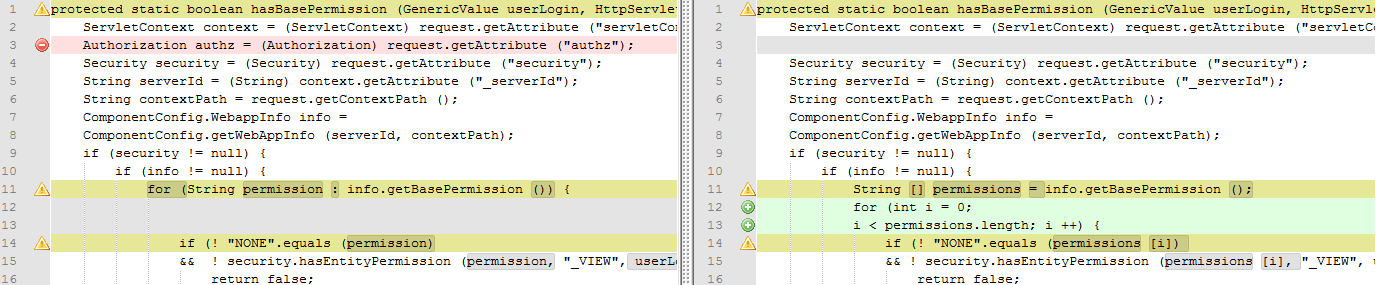
\includegraphics[width=0.9\linewidth]{./img/Permission}
\vspace{-6pt}
\caption{Tactical Clones Detected in Two different Projects}
\label{fig:Permission}
\vspace{-1pt}
\end{figure*}




We then ran concolic analysis on these two code segments which produced the matching concolic output shown in Table~\ref{fig:exampleoutput} which indicated that original code snippets are tactical clone type-4. In this example, variable type integers are represented by a generic tag ``SYMINT.'' Though not present in this example, other variable types are represented in a similar fashion in concolic output. Actual variable names do not appear anywhere in the output and are irrelevant to this clone detection process. We anticipate that open source repositories have a large number of tactical clone type-4 which can be used as items for a recommender system.


In an extensive experiment we ran a leading clone detection tool Nicad~\cite{Roy:2008:NAD:1437898.1438600}, over the tactical code snippets from 37 projects. We chose Nicad for our larger analysis since it is a more mature and refined tool than our experimental technique based upon concolic analysis. However, we believe that concolic analysis represents a more promising technique for tactical clone detection in our future work.




Table~\ref{tab:ChosenProjects} shows tactics used in our study, as well as the number of tactical clones across projects (Note: We do not report tactical clones within the same project). Last column of this table illustrates total number of tactical files used in this study. The tactical clones were detected at method level, although we could have detected them as sub-method level we realized that method level tactical clones are easier to comprehend and therefore easier to reuse for the developers. 


As a result of our explorative study we found several examples of identical tactical code snippets (type1,2 and 3) and several examples of conceptually equivalent tactical code snippets (type 4). Figure \ref{fig:Permission} shows the source code for RBAC tactic across two different projects. In this example two developers in different system have potentially developed the same code snippets to implement the tactic. This observation and several similar detected clones also emphasizes the fact that tactical clones are a more common granularity for code adoption and reuse.



\noindent
\begin{table}[hb] %h for here, t for top, b for bottom
\vspace{-16pt}
\caption{Diff of HeartBeat Concolic Output}
~\label{table:concolicoutputcomparision}
\centering
\begin{tabular}{ p{3.8cm} | p{3.8cm} }
\multicolumn{1}{c}{\textbf{Concolic Segment \#1}} & \multicolumn{1}{c}{\textbf{Concolic Segment \#2}} \\ \hline \hline
\begin{lstlisting}[style=ConcolicOutput]
### PCs: 1 1 0
a_1_SYMINT,
a_1_SYMINT,d1_2_SYMREAL,
a_1_SYMINT,d1_2_SYMREAL,s1_3_SYMSTRING,
\end{lstlisting}
&
\begin{lstlisting}[style=ConcolicOutput]
### PCs: 1 1 0
a_1_SYMINT,
a_1_SYMINT,d1_2_SYMREAL,
a_1_SYMINT,d1_2_SYMREAL,s1_3_SYMSTRING,
\end{lstlisting}

\end{tabular}
\label{fig:exampleoutput}
\vspace{-10pt}
\end{table}

\begin{table}[tbph]
\vspace{-10pt}
\caption{Discovered Tactical Clones Across 37 Projects.}
\label{tab:ChosenProjects}
\centering

%\begin{tabular}{|p{2.0cm}|p{2cm}|p{2.4cm}|}
  \begin{tabular}{ c | l | l }
\hline

\bfseries Tactic & \bfseries Number~of~Clones & \bfseries In~Total~Tactical~Files \\ \hline \hline
Audit & 50    & 352 \\ \hline
Authenticate & 151   & 252 \\\hline
Checkpointing & 8     & 138 \\ \hline
Ping Echo & 10    & 103 \\ \hline
Pooling & 1021  & 1073 \\ \hline
RBAC  & 436   & 477 \\ \hline
Scheduling & 76    & 117 \\ \hline
Secure Session & 249   & 299 \\ \hline
HeartBeat & 0     & 11 \\ \hline
Kerbrose & 0     & 21 \\
\end{tabular}%
\vspace{-10pt}
\end{table}


\section{Conclusion}
In this preliminary work we investigated the challenges toward a robust and practical architecture recommender system. The notion of architectural clones can provide a reusable level of granularity for a recommender system. Our future research will extract tactical clones from thousands of open source system to build an architectural tactic recommender system.
